\chapter{The Netlist: A Wire-Level Blueprint}

\begin{tldr}
\begin{itemize}
  \item \textbf{Last chapter:} PD is a pipeline of engines, each demanding one irreplaceable input. \textbf{This chapter:} we crack open the first input (the netlist) and see the graph the rest of the flow walks across.
  \item A \textbf{netlist} is a textual graph of the design: \textbf{cell instances} as nodes, \textbf{nets} as edges, and \textbf{top-level ports} as the boundary.
  \item \textbf{Synthesis} converts RTL behavior into a netlist of library cells; the same RTL can be re-synthesized into a different technology and produce a different netlist.
  \item Every instance name in a \textbf{synthesized (gate-level) netlist} must resolve to a cell defined in the technology \texttt{.lib}, or the PD tool will throw a missing-reference error before floorplanning even begins.
\end{itemize}
\end{tldr}

\begin{hook}
Hand a physical design tool a million-line netlist and it sees one thing: a giant adjacency list of cells and the wires soldering them together. Strip away the comments, the module wrappers, the friendly signal names, and what is left is a circuit graph. That graph is the only thing the placer, the router, and the timing engine ever really look at. So what does this graph actually say?
\end{hook}

\section{What a Netlist Really Is}

A \textbf{netlist} is a connectivity description. It enumerates the \textbf{components} (cell instances) in the circuit and lists the \textbf{nodes} (nets) that those components share. A \textbf{net} is a single equipotential wire that touches two or more pins. A \textbf{port} is a wire that crosses the module boundary to the outside world.

That is the whole data structure. Three sets: instances, nets, ports. Every PD tool builds the same in-memory graph from whichever text format it was handed.

\begin{keyidea}
A netlist is a \textbf{graph of cell instances connected by nets}, with top-level ports as the only opening to the outside world; everything PD does (placement, routing, timing) operates on this graph.
\end{keyidea}

\section{The 4-Gate Example}

The lecture builds a tiny majority-style circuit with three AND gates feeding one OR gate. The structural picture looks like this.

\begin{figure}[h]
\centering
\begin{tikzpicture}[
  every node/.style={font=\small},
  gate/.style={draw, rectangle, minimum width=10mm, minimum height=8mm, fill=blue!8},
  port/.style={draw, circle, inner sep=1pt, fill=gray!20},
  node distance=8mm
]
  \node[port] (a) at (0,2.4) {a};
  \node[port] (b) at (0,1.2) {b};
  \node[port] (c) at (0,0)   {c};

  \node[gate] (g1) at (2.6,2.1) {g1 AND};
  \node[gate] (g2) at (2.6,0.9) {g2 AND};
  \node[gate] (g3) at (2.6,-0.3) {g3 AND};

  \node[gate] (g4) at (6.0,0.9) {g4 OR};
  \node[port] (cout) at (8.2,0.9) {cout};

  \draw[-Latex] (a)  -- ($(g1.west)+(0,0.15)$);
  \draw[-Latex] (b)  -- ($(g1.west)+(0,-0.15)$);

  \draw[-Latex] (b)  -| ($(g2.west)+(0,0.15)$);
  \draw[-Latex] (c)  -| ($(g2.west)+(0,-0.15)$);

  \draw[-Latex] (a)  to[out=-90,in=180] ($(g3.west)+(0,0.15)$);
  \draw[-Latex] (c)  -- ($(g3.west)+(0,-0.15)$);

  \draw[-Latex] (g1.east) -- node[above,font=\scriptsize] {x} ($(g4.west)+(0,0.25)$);
  \draw[-Latex] (g2.east) -- node[above,font=\scriptsize] {y} (g4.west);
  \draw[-Latex] (g3.east) -- node[below,font=\scriptsize] {z} ($(g4.west)+(0,-0.25)$);

  \draw[-Latex] (g4.east) -- node[above,font=\scriptsize] {cout} (cout);
\end{tikzpicture}
\caption{Structural view of the 4-gate example. Four instances (g1, g2, g3, g4), three internal nets (x, y, z), three input ports (a, b, c), one output port (cout).}
\label{fig:netlist-4gate}
\end{figure}

Count what the graph contains: \textbf{4 instances}, \textbf{3 internal nets}, \textbf{4 ports}. Every wire in the picture maps to exactly one entry in the netlist text.

\begin{hook}
Picture a \textbf{telephone switchboard} where each operator (cell instance) holds labeled cords (pins) and every cord plugs into a single colored wire bundle (net) running across the back panel. Lose one cord-to-bundle mapping and the call drops, which in silicon means the placer refuses to start.
\end{hook}

\section{The Verilog Form}

Here is what the four-gate circuit looks like as a technology-independent Verilog netlist.

\begin{lstlisting}[style=eda,caption={Technology-independent gate-level netlist for the 4-gate example.},label={lst:netlist-gen}]
module maj_block (a, b, c, cout);
  input  a, b, c;
  output cout;
  wire   x, y, z;

  and  g1 (x, a, b);
  and  g2 (y, b, c);
  and  g3 (z, a, c);
  or   g4 (cout, x, y, z);
endmodule
\end{lstlisting}

Read it as three blocks. The \textbf{header} declares ports. The \textbf{wire} statement names internal nets. The body \textbf{instantiates} cells, listing the output pin first and inputs after.

\begin{gut}
In Listing \ref{lst:netlist-gen}, how many \textbf{nets} does the design contain in total (count ports as nets too, since each is a wire crossing the boundary)?
\gutans{Seven: three input ports (a, b, c), one output port (cout), and three internal wires (x, y, z).}
\end{gut}

\section{Technology-Independent vs.\ Synthesized}

The lecture draws a sharp line at the end. The Verilog above uses generic \texttt{and} and \texttt{or} primitives. No PD tool can place those, because they have no area, no pin locations, no drive strength. That version is a \textbf{technology-independent netlist}: pure structure.

A \textbf{synthesized (gate-level) netlist} replaces every primitive with a \textbf{reference} to a real library cell, like \texttt{AND2\_X1} or \texttt{OR3\_X2} from a foundry standard-cell library.

\begin{figure}[h]
\centering
\begin{tikzpicture}[every node/.style={font=\footnotesize}, node distance=6mm]
  \node[draw, rounded corners, fill=red!8, minimum width=42mm, minimum height=22mm, align=left] (rtl) at (0,0)
    {\textbf{RTL Verilog}\\[2pt]
     \texttt{assign cout =}\\
     \texttt{ (a\&b)|(b\&c)|(a\&c);}};
  \node[draw, rounded corners, fill=blue!8, minimum width=42mm, minimum height=22mm, align=left] (gate) at (6.0,0)
    {\textbf{Gate-level netlist}\\[2pt]
     \texttt{AND2\_X1 g1 (.A(a),...);}\\
     \texttt{OR3\_X1  g4 (.A(x),...);}};
  \draw[-Latex, very thick] (rtl) -- node[above] {synthesis} node[below] {(DC, Genus)} (gate);
\end{tikzpicture}
\caption{Before/after: the same intent expressed as behavioral RTL (left) and as a synthesized gate-level netlist bound to library cells (right). PD only consumes the right-hand form.}
\label{fig:rtl-vs-gate}
\end{figure}

The mapping from RTL to gate-level is what the synthesis tool (Design Compiler, Genus, Yosys) does. Same RTL, different \texttt{.lib} target, different netlist. That is why one Verilog source survives a node shrink while the netlist gets thrown out and regenerated.

\begin{hook}
A \textbf{recipe} (RTL) survives moving to a new \textbf{kitchen} (foundry), but the \textbf{ingredient list with brand names} (netlist) gets rewritten every time, and serving the wrong brand (a cell not in the \texttt{.lib}) ruins the whole dish (the PD database refuses to load).
\end{hook}

\begin{pausebox}
Pause. Before reading on, sketch what would happen if your synthesis target was a 7\,nm \texttt{.lib} but you handed PD the netlist synthesized against the 28\,nm library. Where in the flow does the failure show up, and what does the error message complain about?
\end{pausebox}

\section{Why Cell Names Matter (Chapter 9 Foreshadow)}

Every reference name in the synthesized netlist (e.g., \texttt{NAND2\_X2}) is a string lookup into the technology \texttt{.lib}. If the netlist says \texttt{NAND2\_X2} but the library only defines \texttt{NAND2X2} (no underscore), the PD tool reports an unresolved reference and refuses to elaborate the design.

This is why you cannot mix-and-match. The netlist, the \texttt{.lib}, and the LEF (Chapter 9) must all agree on cell names down to the character. We will see in the next chapter why the \texttt{.lib} is the source of truth for those names.

\section{Worked Example: Counting What PD Sees}

\textbf{Problem.} For the netlist in Listing \ref{lst:netlist-gen}, compute the instance count, the net count, and the average net degree (pins per net).

\move{1} \textbf{Instances.} g1, g2, g3, g4 \(\Rightarrow\) \(N_{\text{inst}} = 4\).

\move{2} \textbf{Nets.} Internal: \{x, y, z\}. Port nets: \{a, b, c, cout\}. Total \(N_{\text{net}} = 7\).

\move{3} \textbf{Pin count per net.} Each input port drives certain gates:
\begin{itemize}
  \item \texttt{a}: 1 port + g1.A + g3.A \(\Rightarrow\) 3 pins
  \item \texttt{b}: 1 port + g1.B + g2.A \(\Rightarrow\) 3 pins
  \item \texttt{c}: 1 port + g2.B + g3.B \(\Rightarrow\) 3 pins
  \item \texttt{x}: g1.Z + g4.A \(\Rightarrow\) 2 pins
  \item \texttt{y}: g2.Z + g4.B \(\Rightarrow\) 2 pins
  \item \texttt{z}: g3.Z + g4.C \(\Rightarrow\) 2 pins
  \item \texttt{cout}: g4.Z + 1 port \(\Rightarrow\) 2 pins
\end{itemize}

\move{4} \textbf{Average degree.} Total pins \(= 3+3+3+2+2+2+2 = 17\). Average pins/net \(= 17/7 \approx 2.43\).

\move{5} \textbf{Scaling intuition.} Real SoCs run roughly 1 net per instance. For a 1\,M-instance block, expect on the order of \textbf{1\,M nets}. Each one becomes a routing problem.

\begin{figure}[h]
\centering
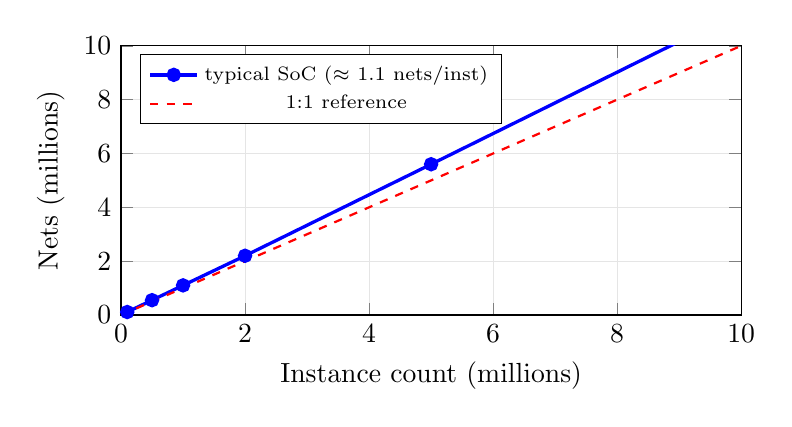
\begin{tikzpicture}
\begin{axis}[
  width=0.78\linewidth, height=5cm,
  xlabel={Instance count (millions)},
  ylabel={Nets (millions)},
  xmin=0, xmax=10, ymin=0, ymax=10,
  grid=both, grid style={gray!20},
  legend pos=north west, legend style={font=\scriptsize}
]
\addplot[blue, very thick, mark=*] coordinates {(0.1,0.11)(0.5,0.55)(1,1.1)(2,2.2)(5,5.6)(10,11.3)};
\addlegendentry{typical SoC ($\approx$ 1.1 nets/inst)}
\addplot[red, dashed, thick] coordinates {(0,0)(10,10)};
\addlegendentry{1:1 reference}
\end{axis}
\end{tikzpicture}
\caption{Net count vs.\ instance count for synthesized blocks. The slope sits slightly above 1 because high-fanout nets (clock, reset, scan-enable) push the average up.}
\label{fig:net-scaling}
\end{figure}

\begin{gut}
For a block with 250{,}000 instances, what is a reasonable first-cut estimate of the net count, and what single signal probably skews that number upward?
\gutans{Around 275{,}000 nets (1.1$\times$ rule). The \textbf{clock net} typically touches every flop, but it gets split into a tree by CTS so the raw netlist still shows it as one giant net.}
\end{gut}

\begin{pitfall}
\textbf{Common netlist misconceptions.}
\begin{itemize}
  \item \textbf{Behavioral vs.\ structural.} A file with \texttt{always} blocks or \texttt{assign} expressions is \emph{not} a netlist PD can consume. PD wants pure structural Verilog: instances and connections only.
  \item \textbf{Blackboxes.} An instance whose module body is not in the netlist (memories, hard macros, IP blocks) is a \textbf{blackbox}. PD still needs its physical view (LEF) and timing view (\texttt{.lib}); otherwise it cannot place or time around it.
  \item \textbf{Cell name mismatch.} \texttt{INVX1} in the netlist will not bind to \texttt{INV\_X1} in the \texttt{.lib}. Spelling, case, and underscores all matter.
  \item \textbf{Non-uniquified hierarchical netlists.} If the same module is instantiated under two parents that need different constraints (say, one on a critical 1\,GHz datapath, the other in scan-only logic), synthesis must \textbf{uniquify} by renaming each instance to a distinct module. A non-uniquified netlist applies one set of timing budgets to both, and the failing endpoint shows up only at signoff, after a week of PD work.
  \item \textbf{Physical-only cells without \texttt{.lib} entries.} Tap cells, end-caps, decaps, and ECO fillers live in the netlist (or get inserted post-synthesis) but have no timing arcs in \texttt{.lib}. PD tools handle this gracefully; STA-only flows can throw confusing missing-pin errors if the engineer forgot to mark them as physical-only.
\end{itemize}
\end{pitfall}

\begin{sidebar}
\textbf{Hierarchical vs.\ flat netlists.} A hierarchical netlist preserves module boundaries (\texttt{cpu/alu/adder/g1}); a flat netlist dissolves them so every leaf instance lives at the top (\texttt{cpu\_alu\_adder\_g1}). Hierarchical is easier for humans and faster to elaborate; flat gives the optimizer freedom to retime and resize across former boundaries. Most modern flows stay hierarchical at top and flatten selectively inside each block.

\textbf{EDIF.} Older flows and some FPGA tools exchange netlists in \textbf{EDIF} (Electronic Design Interchange Format), a Lisp-like S-expression syntax. The information is identical; the grammar is just uglier. ASIC PD today is overwhelmingly Verilog.
\end{sidebar}

\begin{pdnote}
\textbf{Why PD cares.}
\begin{itemize}
  \item \textbf{ARM PD internship lens:} the first thing you do on day one is load a synthesized \texttt{.v} into Innovus or ICC2 and check that every reference resolves against the loaded \texttt{.lib}/LEF; unresolved references are the most common ``my flow won't start'' ticket.
  \item \textbf{Generic foundry-flow PD engineer lens:} the netlist drives \textbf{instance count budgeting} (placement density), \textbf{net count budgeting} (routing congestion), and \textbf{port count budgeting} (pin planning at block boundaries); all three pop out of a 30-second \texttt{report\_design} run.
  \item \textbf{VLSI interview lens:} expect ``what is the difference between a behavioral and a structural netlist?'' and ``which inputs does PD need before placement?''; the netlist is always one of the three answers (netlist, \texttt{.lib}, LEF).
\end{itemize}
\end{pdnote}

\begin{checkpoint}
You should now be able to: (1) define a netlist as an instance/net/port graph, (2) distinguish a technology-independent netlist from a synthesized one, (3) read a small Verilog gate-level netlist and count instances and nets, and (4) explain why every reference in the netlist must match a cell in the \texttt{.lib}.

\mnemonic{INP: Instances, Nets, Ports}
\end{checkpoint}
